\part{Praktická část}

\chapter{Cíl projektu}

V~praktické části mé práce jsem vytvořil vlastní hru pro VR. Stanovil jsem si následující kritéria:

\begin{itemize}
  \item \textbf{Nenáročnost}. Chtěl jsem, aby má hra nebyla obtížná na pochopení. Většina VR her vyžaduje zvýšenou fyzickou aktivitu nebo hlubší porozumění VR konceptů. Ideálně jsem chtěl vytvořit hru, kterou bych mohl komukoliv půjčit, aniž bych musel dlouze vysvětlovat její princip.
  \item \textbf{Grafická jednoduchost}. Nepovažuji se za umělce a umím vytvářet pouze základní modely a textury. Bylo pro mě tedy klíčové přijít s~takovým konceptem, který by byl vzhledově nenáročný.
  \item \textbf{Interaktivita}. Od své hry jsem chtěl, aby doopravdy využívala funkce, které VR platformy poskytují. Tedy ovládání pohybem, vliv fyzikálních zákonů atp.
\end{itemize}

\begin{quotation}
  
\textbf{Dospěl jsem k~následujícímu nápadu}: Logická hra sestávající z~kostky tvořené úrovněmi naskládanými na sebe. Každá úroveň představuje bludiště, skrze které musí nakláněním hráč navigovat kuličku. Při dosažení cíle je úroveň odebrána, kostka se zmenší a je odhalena další úroveň.
\end{quotation}

Toto splňuje moje kritéria \poml hra je jednoduchá, na vykreslení potřebuje jen geometrické tvary a vyžaduje pohyb rukama pro naklánění bludiště.

Výsledný projekt je složen z~mnoha souborů, mnoho z~nichž nejsou kód a není vhodné je do textu práce zahrnout. 

Celý zdrojový kód je veřejnosti dostupný na adrese \url{https://github.com/sykdan/puzzle_prism/tree/mprace}. 

\chapter{Struktura projektu}

\begin{samepage}
  Můj projekt jsem rozdělil do jednotlivých, jednoduše spravovatelných scén. Tímto jsem mohl na mnohých funkcích pracovat odděleně a mohl bych je teoreticky použít i v~budoucích projektech. Zde je zjednodušený diagram těchto scén:

  \begin{figure}[H]
    \centering
    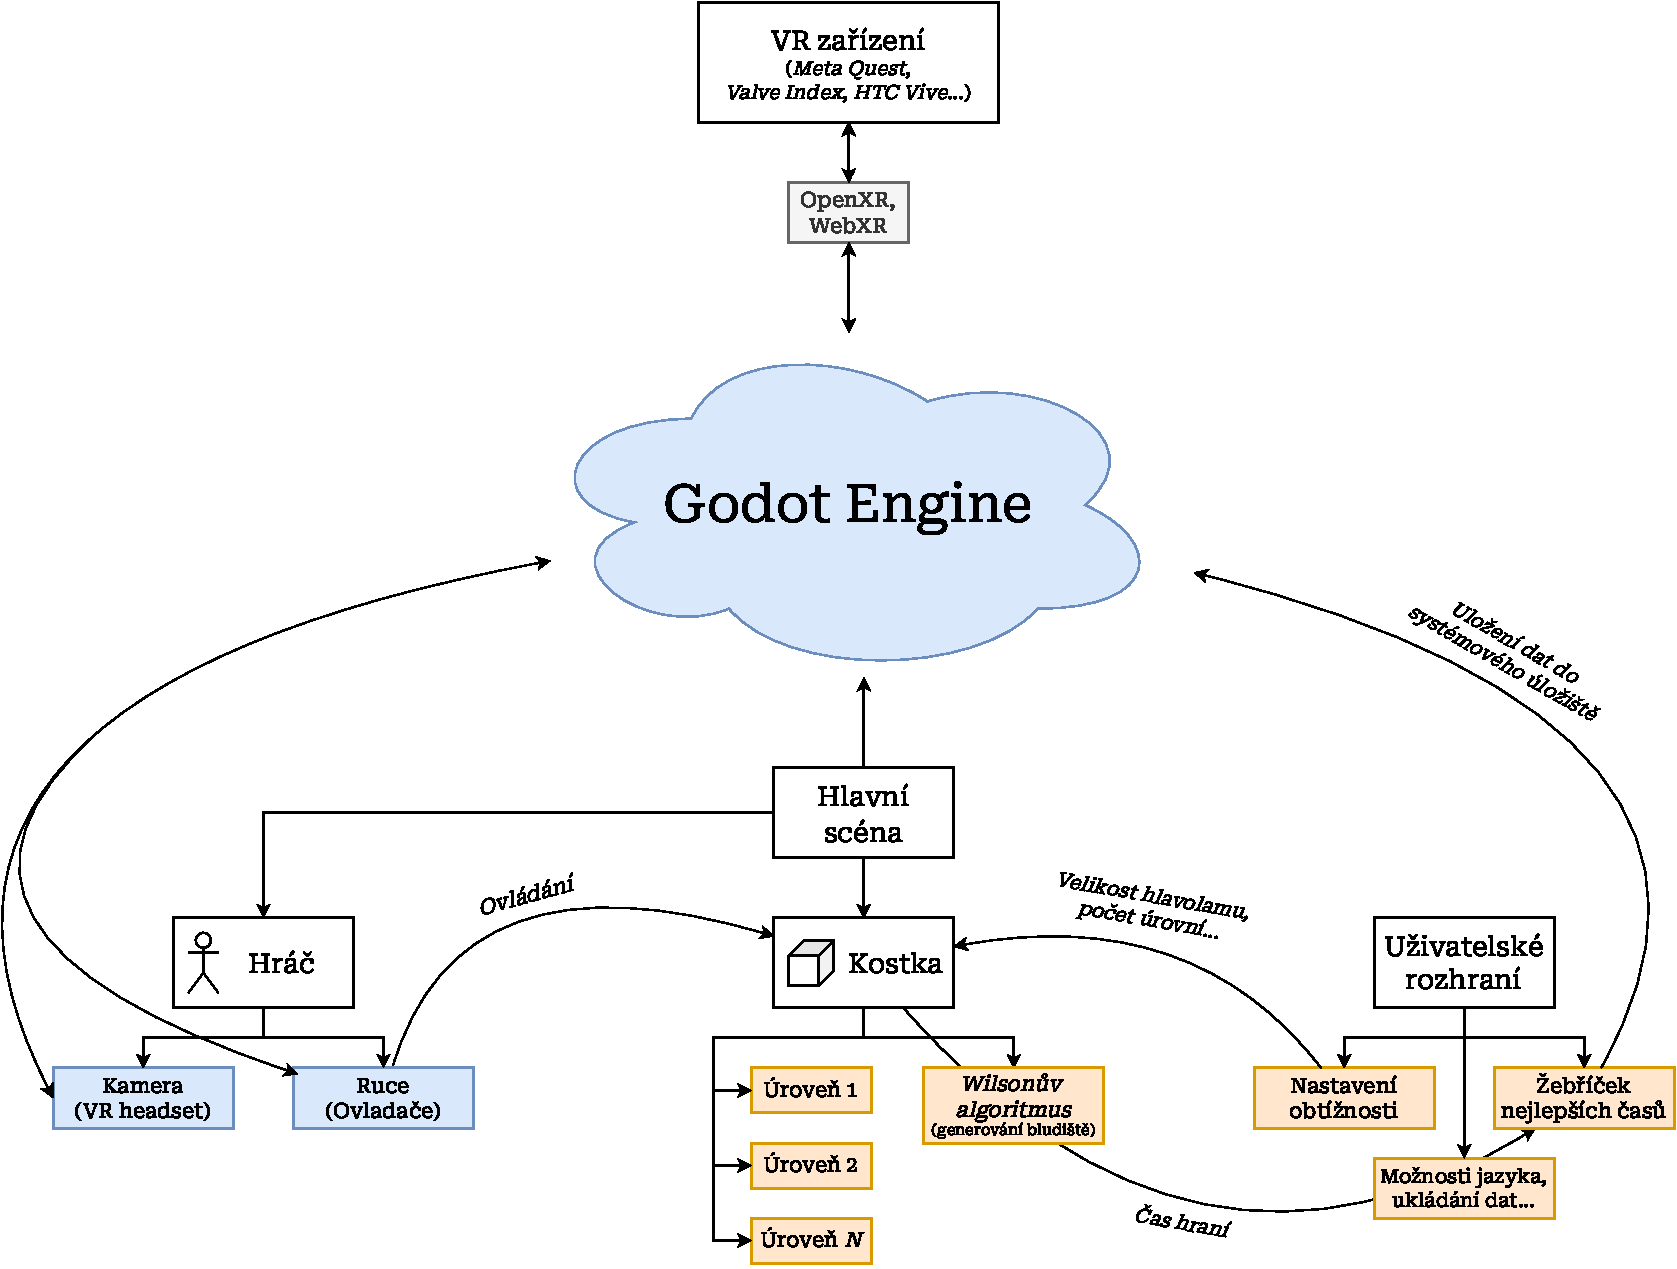
\includegraphics[width=\linewidth]{diagram.pdf}
    \caption{Diagram scén a tok dat mezi nimi}
  \end{figure}
\end{samepage}


\begin{figure}[H]
  \vspace{1em}
  \hrule
  \vspace{1em}

  \renewcommand\DTstyle{\sffamily}
  \dirtree{%
    .1 Hlavní scéna (spojuje a ovládá zbylé scény) .
    .2 Prostředí (skybox \poml pozadí, osvětlení) .
    .2 Hráč .
    .3 Trackované ovladače, kamera synchronizovaná s~headsetem .
    .2 Obrazovka .
    .3 Výběr obtížnosti, žebříček nejlepších, nastavení hry .
    .2 Kostka s~bludištěm .
    .3 Kostka o~určité velikosti .
    .4 Úroveň (bludiště, ze kterých se kostka skládá) .
    .5 Komnata (buňky, ze kterých se skládá bludiště) .
    .3 Kulička (volně se pohybující předmět s~vlastní fyzikou) .
  }
  \vspace{1em}
  \hrule
  \vspace{1em}
  \caption{Podrobný strom scén}
\end{figure}

Každá scéna reprezentuje odlišnou sadu problémů a výzev, které jsem musel při tvorbě projektu řešit.

\section{Hráč, interakce se zařízením}

Scéna s~hráčem je přímo spojena s~headsetem a sledovanými ovladači. Sestává z~uzlů \texttt{XRCamera3D}, pohledu do 3D prostředí synchronizovaným s~umístěním headsetu, a dvou uzlů \texttt{XRController3D}, které jsou synchronizované s~umístěním levého a pravého ovladače.

V~této scéně jsem použil svobodnou knihovnu \textit{Godot XR Tools}, která nabízí podpůrné scény pro XR projekty. Z~té jsem si zapůjčil kód nutný k~inicializaci VR headsetu a 3D model ruky licencovaný pod \textit{Creative Commons 0}\footnote{CC0 je licence používaná pro díla ve veřejné doméně. Autoři modelu se vzdali autorských práv. Vizte \url{https://creativecommons.org/publicdomain/zero/1.0/deed.cs}}.

Od přátel, kteří hru testovali, jsem často slýchal stížnosti, že jim hra způsobuje nevolnost. Přidal jsem proto do této scény i platformu, umístěnou pod hráčem ve výšce, kterou si ve svém zařízení předem nastavil jako výšku podlahy. Mým záměrem bylo zabránit pocitu, že se hráč \uv{vznáší v~prázdnotě}, čímž bych nepříjemný pocit odstranil. Testující na změnu reagovali pozitivně. 

Účel scény je kromě správného zobrazení hry také interpretace vstupu od hráče. Ve hře jsou klíčové dvě funkce: uchopení nějakého předmětu (např. kostky pro její naklánění) a interakce s~uživatelským rozhraním pomocí laserového ukazovátka. Druhý zmíněný bod popisuji podrobněji v~sekci \ref{uzivatelske_rozhrani}.

Implementovat uchopení předmětu \textit{jednou rukou} je triviální \poml Stačí, aby tento objekt sledoval změny v~transformaci uzlu \texttt{XRController3D}. Uchopení \textit{oběma rukama}, chování, kterého jsem chtěl dosáhnout ve své hře, je ale složitější. Protože je možné ovladače volně pohybovat a neexistují žádná fyzická omezení (hráč by mohl předmět např. volně kroutit), musel jsem přistoupit ke kompromisu. Při sevření tlačítek na obou ovladačích hra vytvoří třetí, neviditelný ovladač. Tento ovladač působí ze středu mezi levým a pravým ovladačem a je rotován tak, aby vektor Z~tranformační matice\footnote{Godot Engine používá pro rotaci uzlů transformační matice. Vektor Y míří vzhůru.} mířil od levého ovladače k~pravému ovladači a vektor Y mířil stejným směrem jako palce uživatele. Hra se poté odkazuje na tento virutální ovladač. Výsledný efekt je velmi přesvědčivý. Celá implementace této logiky je vložena v~příloze \ref{apx_gripped_object_transformation}.

\section{Kostka, bludiště}

Kostka je hlavním prvkem hry. Jedná se o~dutou kostku s~průhledným víkem, ve které je několik úrovní (bludišť) a kulička. Každé bludiště je v~podstatě mřížka čtvercových buněk, které jsou odděleny zdmi. Cílem je manipulováním s~kostkou dostat kuličku k~vlajce, načež kulička propadne o~úroveň níž a kostka se zmenší.

Hlavní výzvou v~této scéně je vygenerování náhodného bludiště, aby bylo možné hru hrát donekonečna.

\begin{figure}[H]
  \centering
  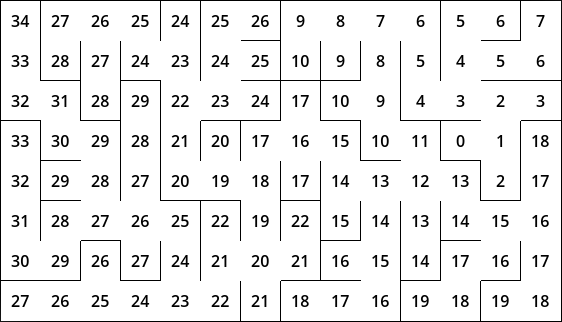
\includegraphics[height=180pt]{maze_example.png}
  \caption{Ukázka vygenerovaného bludiště (v~2D podobě) z~testovací scény}
  \label{maze_example}
\end{figure}

Pro vygenerování bludiště jsem použil \textit{\textbf{Wilsonův algoritmus}}. Důvodem je fakt, že tento algoritmus nemá sklony vytvářet extrémně dlouhé či extrémně krátké chodby, na rozdíl od jiných algoritmů. Postup je následující: \cite{enwiki:1193338583}

\begin{enumerate}
  \setcounter{enumi}{0}
  \item Mějme graf buněk, kde má každá buňka několik sousedních buněk (např. pro mřížku mají buňky 4 sousední buňky, vyjma těch na krajích a v~rozích). Nechť je mezi všemi sousedícími buňkami spojení, které lze označit jako průchod nebo zeď.
  \item Označme všechny spojení jako zdi a jednu náhodně zvolenou buňku označme jako zahrnutou v~bludišti. \label{init}
  \item Libovolným způsobem zvolme buňku. Pokud je tato buňka zahrnuta v~bludišti, zvolme jinou buňku. \label{pick}
  \item Označme buňku jako zahrnutou v~současné iteraci.
  \item Přejděme na náhodnou sousedící buňku a v~předchozí buňce uložíme ukazatel k~následující buňce. Poté: \label{lerw}
        \begin{itemize}
          \item Pokud tato buňka není zahrnuta ani v~iteraci, ani v~bludišti, označme ji jako zahrnutou v~iteraci a přejděme na krok \ref{lerw}.
          \item Pokud je tato buňka zahrnuta v~iteraci, vznikla smyčka. Pomocí ukazatelů uložených v~buňkách projděme tuto smyčku, odstraňme buňky ze současné iterace a odeberme ukazatele.
          \item Pokud je tato buňka zahrnuta v~bludišti, všechny buňky v~iteraci označme jako buňky v~bludišti. Spoje mezi buňkami v~této iteraci označme jako průchody.
        \end{itemize}
  \item Pokud stále existují buňky, které nejsou zahrnuty v~bludišti, přejděme zpět ke kroku \ref{pick}.
\end{enumerate}

\begin{figure}[H]
  \centering

  \begin{minipage}{.5\textwidth}
    \centering
    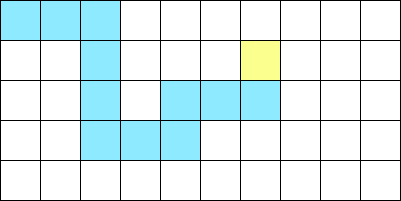
\includegraphics[height=100pt]{maze_gen_step_1.png}
  \end{minipage}%
  \begin{minipage}{.5\textwidth}
    \centering
    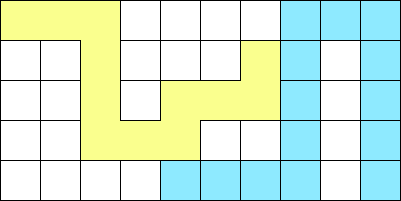
\includegraphics[height=100pt]{maze_gen_step_2.png}
  \end{minipage}

  \caption{Příklad dvou iterací kroků \ref{pick} až \ref{lerw}. Žlutě jsou zvýrazněny buňky v~bludišti, modře buňky v~iteraci.}
\end{figure}

\begin{figure}[H]
  \centering
  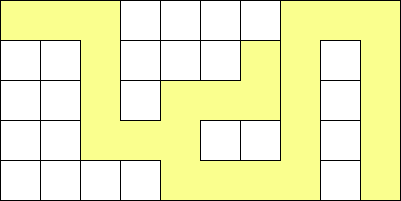
\includegraphics[height=120pt]{maze_gen_step_3.png}
  \caption{Stav po těchto dvou iteracích}
\end{figure}

Takto vygenerované bludiště nemá žádný začátek ani konec; je stvořené z~náhodně propletených buněk. V~prvních verzích hry byl konec náhodně zvolený, docházelo ale k~situacím, kdy byl konec velmi blízko počáteční pozici. Algoritmus jsem proto upravil, aby zároveň zaznamenával vzdálenost od úvodní buňky (viz krok \ref{init}). Jelikož výběr úvodní buňky nemá na výsledek algoritmu vliv, umožnil jsem explicitně zadat její pozici. Úvodní buňku teď můžu považovat za začátek bludiště, a nejvzdálenější buňku jako konec. Celá implementace algoritmu je uvedena v~příloze \ref{apx_mazegen}.

\begin{figure}[H]
  \centering

  \begin{minipage}{.5\textwidth}
    \centering
    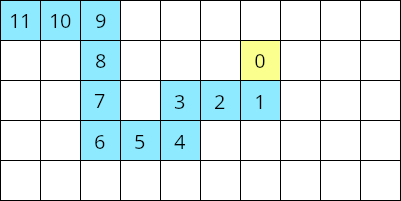
\includegraphics[height=100pt]{maze_gen_count_1.png}
  \end{minipage}%
  \begin{minipage}{.5\textwidth}
    \centering
    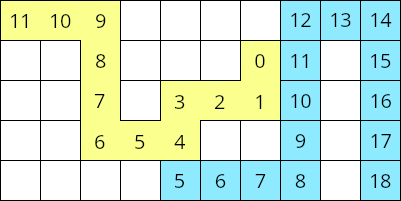
\includegraphics[height=100pt]{maze_gen_count_2.png}
  \end{minipage}

  \caption{Počítání vzdálenosti paralelně s~generováním}
\end{figure}

Po vygenerování bludiště hra podle výsledných dat postaví bludiště. Instancuje scénu s~úrovní a v~jednotlivých komnatách připraví zdi. Aby se zabránilo dlouhým načítacím dobám, lze hru hrát již po vygenerování dvou úrovní. Zbytek je generován a doplněn na pozadí, předpokládá se, že hráč bude hrát pomaleji, než se hra generuje.

Druhou výzvou je samotná fyzika kuličky. Godot Engine nabízí modul pro simulaci fyziky, kterého jsem využil. Kuličku tvoří uzel \texttt{RigidBody3D} (tuhé těleso) a stěny uzel \texttt{StaticBody3D} (nehybné těleso). Fyzika je následně procesována automaticky. Přidal jsem však haptickou odezvu při srážce kuličky se stěnou bludiště \poml při prudké změně v~rychlosti kulička vyšle signál se sílou vibrace, který hlavní scéna zaznamená a ve scéně s~hráčem vyvolá slabou vibraci v~ovladačích.

\begin{figure}[H]
  \centering
  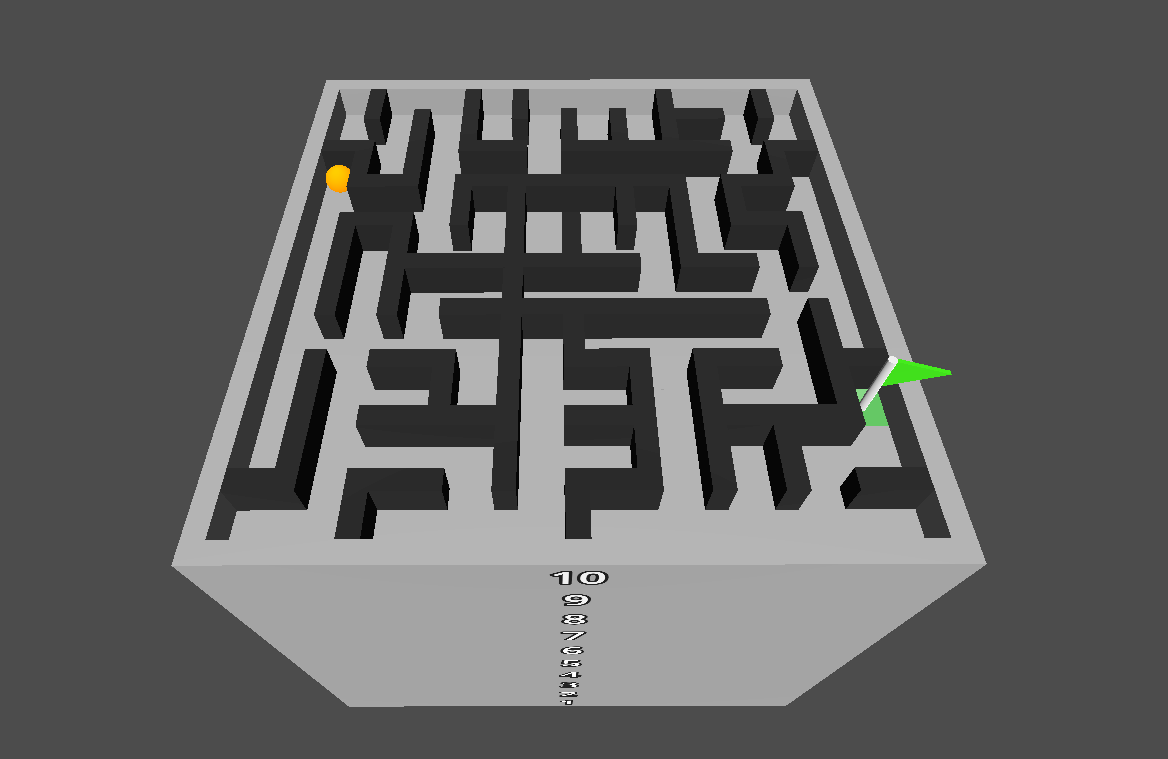
\includegraphics[height=180pt]{maze.png}
  \caption{Celá kostka}
  \label{maze_fig}
\end{figure}

\label{uzivatelske_rozhrani}
\section{Uživatelské rozhraní}

Grafické uživatelské rozhraní je nedílnou součástí každé aplikace nebo hry. Ve VR ovšem nemáme k~dispozici myš ani klávesnici, vše je ovládáno pohybem. Přesto je ale možné dosáhnout podobného chování, jaké známe z~tradičních rozhraní. Většina VR softwaru používá pro své rozhraní virtuální \uv{obrazovky}, plošiny, které zobrazují 2D obsah podobně jako monitor. Uživatel poté využívá virtuální \uv{laserové ukazovátko}, kterým na tyto obrazovky ukazuje a stisknutím tlačítka s~nimi interaguje.

\begin{figure}[H]
  \centering
  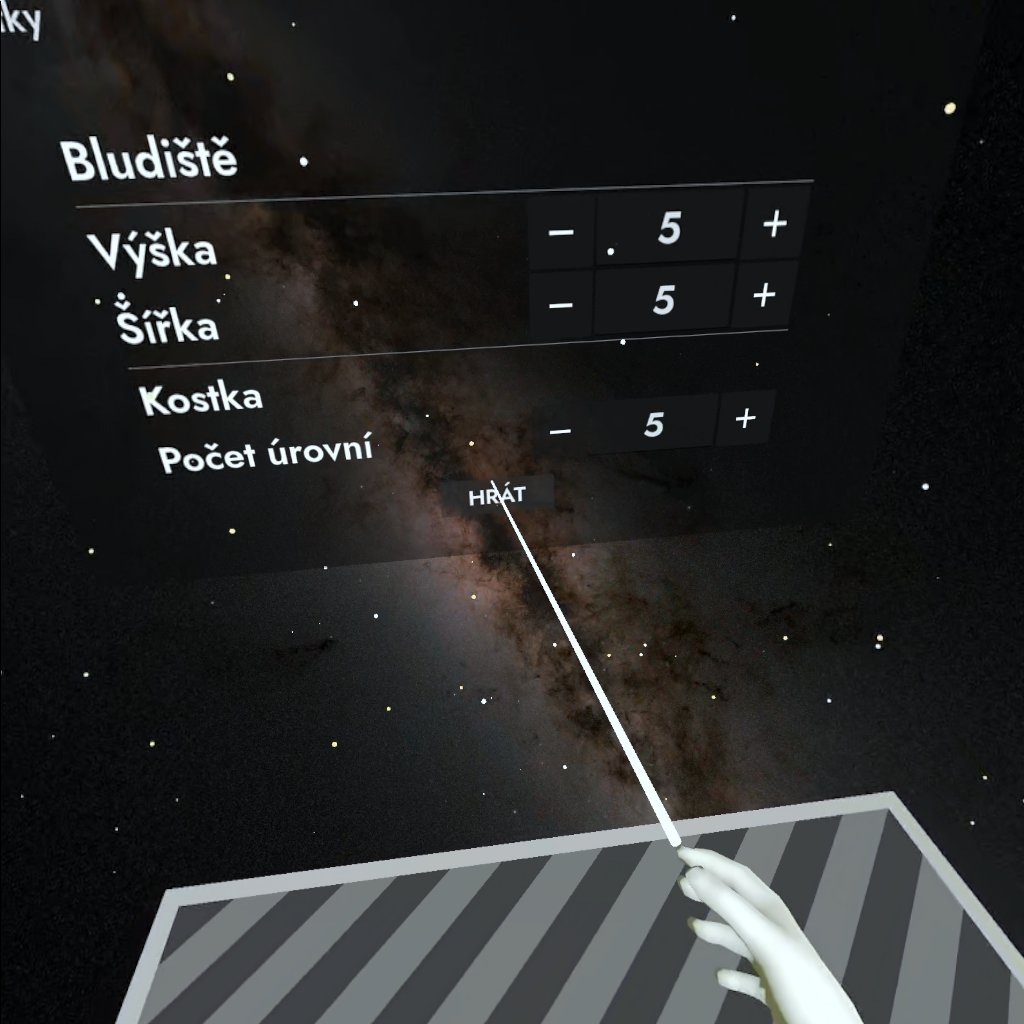
\includegraphics[height=220pt]{game_gui_screenshot.png}
  \caption{Ukázka rozhraní hry. Uživatelova pravá ruka je vybavena ukazovátkem, kterým může vybírat možnosti na obrazovce.}
  \label{game_gui_screenshot}
\end{figure}

Pro vykreslení orbazovky jsem použil uzel \texttt{SubViewport}, který umožňuje vytvořit virtuální plátno a libovolně ho v~rámci enginu zobrazit. Tomuto uzlu můžu přiřadit libovolné dceřinné uzly, které jsou poté renderovány do tohoto plátna. Samo o~sobě není vidět, ale může být přiřazeno jako textura k~jinému uzlu. Pro můj účel jsem použil uzel \texttt{MeshInstance} (instance 3D objektu) a jako objekt použil jednoduchý obdélník.

Interakce s~obrazovkou využívá postup zvaný \textit{ray casting}, česky \textit{vysílání paprsků}. Z~ruky hráče vyšleme paprsek směrem, kterým ukazuje, a při kolizi s~nějakým objektem (v~tomto případě obrazovkou) vypočítáme pozici, kde ke kolizi došlo. Godot Engine má podporu pro ray casting v~rámci uzlu \texttt{RayCast3D}, který jsem přidal do scény s~hráčem. Pokud tento uzel zaznamená kolizi se scénou Obrazovka, zobrazí paprsek mířící od prstu hráče k~obrazovce a začne v~jejím \texttt{SubViewport}u simulovat vstup myší. Simulování vstupu mi umožňuje využít nespočet vestavěných uzlů pro tvorbu rozhraní.

\chapter{Scénář hry}

Při vstupu do hry se hráč ocitne v~hlavní nabídce. Ta je koncipovaná co nejjednodušeji \poml hráči jsou ihned představeny čtyři herní režimy, stupňované dle komplexity.

\begin{itemize}
  \item \textbf{Lehká obtížnost} \poml Bludiště má rozměry 5x5 buněk a kostka má 5 úrovní.
  \item \textbf{Střední obtížnost} \poml Bludiště má rozměry 8x8 buněk a kostka má 8 úrovní.
  \item \textbf{Těžká obtížnost} \poml Bludiště má rozměry 14x14 buněk a kostka má 14 úrovní.
  \item \textbf{Vlastní} \poml Hráč si může volně přizpůsobit rozměry hry.
\end{itemize}

K~dispozici jsou i menší, méně důležitá tlačítka pro vstup do nastavení, ukončení hry a zobrazení návodu. Návod se hráči otevře také při úplně prvním spuštění hry.

U~všech režimů hra zaznamenává čas, za jaký byl hráč schopný hlavolam vyřešit. Přednastavené obtížnosti (lehká, střední, těžká) taktéž ukládají pět nejlepších výsledků. Pokud hráč pokoří jeden z~těchto rekordů, dostane možnost zadat své jméno a uložit tím svůj čas.